\chapter{Propuesta}\label{chapter:proposal}

En este capítulo se presenta un sistema que permite la resolución automática de problemas de clasificación arbitrarios.
Este sistema tiene entre sus objetivos fundamentales producir clasificadores que sean justos respecto a una o varias métricas de equidad, a la vez que minimizan una función de perdida determinada.
Para ello se propone un enfoque dividido en dos fases, que utiliza una combinación de técnicas de \emph{AutoML}, métodos de ensemble y optimización multiobjetivo.
La sección~\ref{section:overview} provee una descripción general del sistema.
Las secciones~\ref{section:first-phase} y~\ref{section:second-phase} detalla el funcionamiento de la primera y segunda fase del sistema respectivamente.

\section{Descripción general}\label{section:overview}

El sistema toma como entrada una colección de datos $D = \{(x_1, y_1), \dots , (x_n, y_n)\}$, una función de pérdida $\mathcal{L}$ y una o varias métricas de equidad $F_1, F_2, \dots, F_n$.
El objetivo del sistema es producir un modelo de clasificación que es a la vez efectivo según $L$ y justo según $F_1, F_2, \dots, F_n$.
El sistema consiste en dos fases fundamentales.
La primera es responsable de generar una colección de modelos, cada uno llamado modelo base.
Esta colección es construida optimizando la función de perdida $\mathcal{L}$, mientras se asegura \emph{diversidad} a lo largo de toda la población.
La segunda fase es responsable de producir un conjunto de modelos de clasificación.
Estos modelos son generados ensamblando la colección de modelos base de forma tal que optimice su efectividad según $L$, a la vez que es lo más \emph{justo} posible según $F_1, F_2, \dots, F_n$.
La figura~\ref{fig:overview} resume la arquitectura del sistema.
Las secciones \ref{section:first-phase} y \ref{section:second-phase} abordan con más detalles la primera y segunda fase, respectivamente.

\begin{figure}[h]
    \begin{center}
        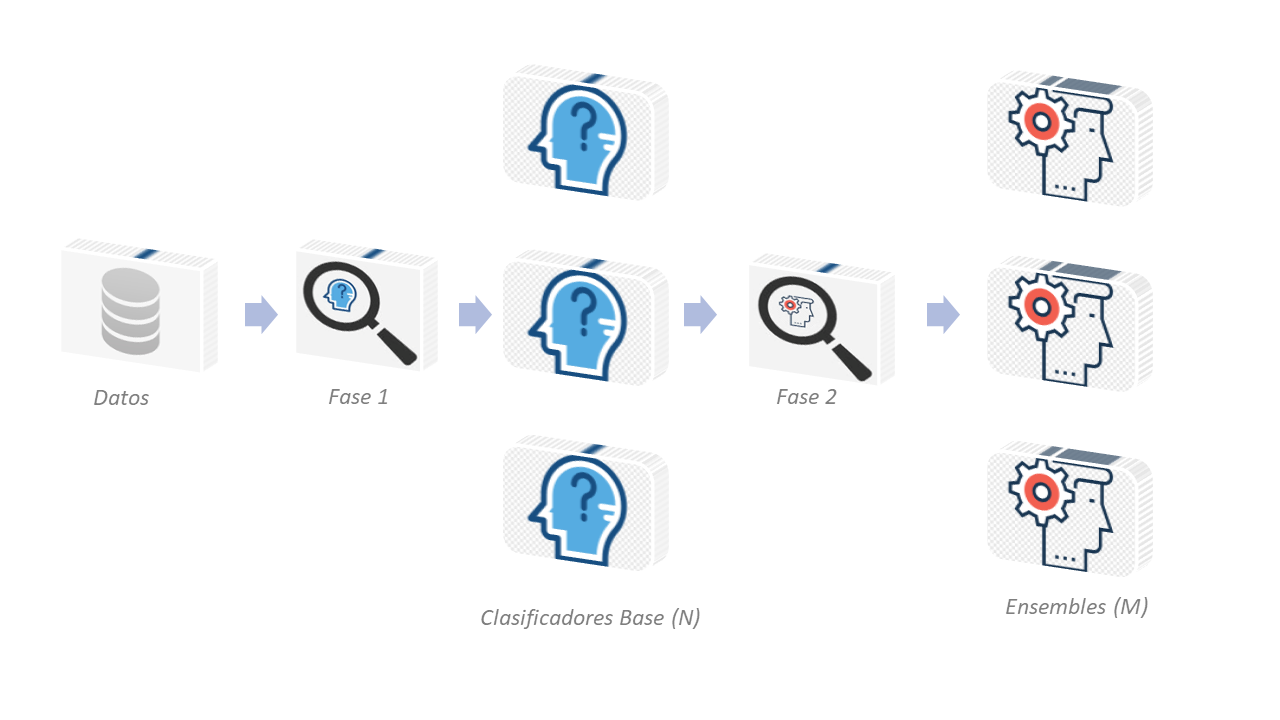
\includegraphics[width=0.9\textwidth]{Graphics/overview.png}
    \end{center}
    \caption{Descripción general del funcionamiento de extremo a extremo del sistema.}
    \label{fig:overview}
\end{figure}

% TODO
% Figure 1 summarizes the architecture of the system.
% Figure 2 and 3 provide an overview of the first and second phase, respectively.

\section{Fase 1: Generación de modelos base}\label{section:first-phase}

% TODO
% Figure 2 provides an overview of this phase.
% Algoritmo

En esta fase, al sistema se le da la tarea de generar $N$ modelos para ajustar $D$ de acuerdo a la pérdida $\mathcal{L}$.

La Definición~\ref{definition:cash} se modifica para buscar una colección de modelos en lugar de un solo modelo, sujeto a una métrica de diversidad $\mathcal{D}$.
Esto es, se desea encontrar una colección de modelos base (modelos que optimicen la efectividad en el conjunto de datos $D$ de acuerdo a la función de pérdida $\mathcal{L}$) mientras garantiza algunas diferencias entre sus hipótesis utilizando la métrica $\mathcal{D}$.
Asegurar diversidad en la colección de modelos base es importante porque los métodos de ensemble no son capaces de mejorar su rendimiento si todos los modelos base tienen exactamente la misma hipótesis, es decir, si todos realizan las mismas predicciones.

El procedimiento aplicado para generar la colección de modelos base esta resumido por la función \ref{code:generate-base-models}.
El espacio de algoritmos e hiperparámetros es explorado utilizando una estrategia de búsqueda preseleccionada.
Todo esto es capturado por la función \textbf{explore}.
Luego de (1) evaluar las arquitecturas generadas y (2) estimar la diversidad entre los modelos actualmente seleccionados y la nueva generación de modelos, la colección de modelos base es actualizada para ajustarse a su capacidad $N$.
Todo esto es capturado por la función \ref{code:reselect}.

\begin{algorithm}[!ht]
    \caption{GenerateBaseModels($N, D, A, \Lambda, \mathcal{L}, \mathcal{D}$)\label{code:generate-base-models}}
    \SetKwData{output}{base\_models}
    \SetKwData{score}{scores}
    \SetKwData{diversity}{diversity}
    \SetKwData{generation}{generation}
    \SetKwData{init}{\bf set}
    \SetKwData{sample}{\bf explore}
    \SetKwData{reselect}{\textbf{\ref{code:reselect}}}

    \init $\output \leftarrow \emptyset$ \\
    \For{$\generation \in \sample(A, \Lambda)$}{
        $\score \leftarrow \emptyset$ \\
        \For{$A^{(j)}_\lambda \in \generation$}{
            $\score^{(j)} \leftarrow \frac{1}{K} \sum_{i=1}^{K} \mathcal{L}(A^{(j)}_\lambda,\ D^{(i)}_{train},\ D^{(i)}_{valid})$ \\
        }
        $\diversity \leftarrow \mathcal{D}(\output \frown \generation,\ D)$ \\
        $\output \leftarrow \reselect(\output \frown \generation,\,\score,\,\diversity,\,N$)
    }
    \Return{\output}
\end{algorithm}

% TODO Probablemente la parte de PGE queremos pasarla para el estado del arte
Para explorar inteligentemente  el espacio de algoritmos e hiperparámetros, es decir, para resolver el problema \textit{CASH} modificado, se utiliza la implementación de \emph{Probabilistic Grammatical Evolution Search}~(algoritmo \ref{algorithm:pge}) presente en AutoGOAL.
La búsqueda comienza con una estrategia de muestreo aleatorio, pero según evalúa más flujos, modifica el modelo de muestreo probabilístico para que flujos similares a los mejores encontrados hasta el momento, sean generados con mayor frecuencia.
El espacio de algoritmos e hiperparámetros empleado es el utilizado por defecto en AutoGOAL, el cual incluye varios algoritmos clásicos de aprendizaje automático presentes en las diferentes bibliotecas utilizadas por AutoGOAL.

% TODO Linkear aqui a recomendaciones de como mejorar la seleccion del conjunto más diverso
Para reseleccionar la colección de modelos base, o sea, la colección de flujos de AutoGOAL, un enfoque goloso es utilizado.
La función \ref{code:reselect} resume la estrategia propuesta.
El algoritmo siempre incluye el modelo que mejor se desempeña de acuerdo a $\mathcal{L}$ en la selección. Cada iteración siguiente añade el modelo, todavía no seleccionado, que maximiza la diversidad respecto a todos los modelos anteriormente seleccionados.
El enfoque goloso no garantiza que la colección final logre la mejor posible diversidad respecto a $\mathcal{D}$.
La precisión tampoco es tomada en cuenta, excepto para seleccionar el modelo de mejor desempeño.

\begin{algorithm}[!ht]
    \caption{reselect($M,\ scores,\ diversity,\ N$)\label{code:reselect}}
    \SetKwData{init}{\bf inicializar}

    \init $R \leftarrow \emptyset$ \\
    \init $R^{(0)} \leftarrow \underset{m^{(j)} \in M}{argmin}$ $scores^{(j)}$ \\
    \For{$r \leftarrow 1\ \KwTo\ N$}{
       $R^{(r)} \leftarrow \underset{(m^{(j)} \in M \setminus R)}{argmax}\ \underset{(m^{(i)} \in R)}{\sum} diversity^{(i,j)}$
    }

    \Return{$R^{(0)} \cdots R^{(N)}$}
\end{algorithm}

Utilizando el enfoque goloso presentado anteriormente, tres implementaciones de referencia del método~\ref{code:reselect} son descritas a continuación.
Estas servirán para establecer comparaciones con implementaciones en las cuales se utiliza el método goloso presentado anteriormente, variando la métrica de equidad del mismo para utilizar \textit{disagreement} y \textit{double-fault}, las cuales serán presentadas en la sección~\ref{section:diversity-meassures}.

\begin{description}
    \item[Shuffle:]
    La colección de modelos base es construida barajando aleatoriamente la selección actual de modelos base y los nuevos encontrados.
    Los primeros $N$ modelos luego de barajar son seleccionados para la siguiente generación.
    \item[Arbitrary:]
    La colección de modelos base es construida de la misma forma que con la estrategia \textit{shuffle}, pero el modelo de mejor rendimiento siempre es incluido en la colección de modelos base seleccionados.
    \item[Best:]
    La colección de modelos base es construida a partir de seleccionar los modelos de mejor rendimiento entre los previamente seleccionados y los recién encontrados.
\end{description}

A continuación, la sección~\ref{section:diversity-meassures} provee algunos detalles acerca de las métricas de diversidad estudiadas en este trabajo.

\subsection{Métricas de diversidad}\label{section:diversity-meassures}

Dos métricas fueron implementadas para estimar la diversidad de una colección dada de modelos base.
Ambas de ellas precomputan una matriz de clasificaciones incorrectas, la cual es utilizada entonces para computar una métrica que aporta información sobre la diversidad entre los modelos base dos a dos.
La matriz de clasificaciones incorrectas se construye de la siguiente manera.

\begin{equation}
    M_{i,j} =
    \begin{cases}
        1 & \text{si el modelo j correctamente clasifica el ejemplo i ($D_{valid}$)} \\
        -1 & \text{en otro caso}
    \end{cases}
\end{equation}

Las siguientes métricas son computadas entre pares de modelos base para estimar cuan diferentes son sus hipótesis, y por tanto la diversidad de la colección incluyendo a ambos a la vez.

\begin{description}

    \item[Disagreement.]
    Esta mide la frecuencia con la cual uno de los modelos falla cuando el otro no lo hace, y viceversa.
    Mientras más alto el valor de la métrica, más diferentes son los modelos.

    \begin{equation}
        \texttt{disagreement}(m^{(a)}, m^{(b)}) = \frac{\vert\{M_{i,a} \neq M{i,b} \vert s^{(i)} \in D^{(\star)}_{valid}\}\vert}{\vert D^{(\star)}_{valid} \vert}
    \end{equation}

    \item[Double Fault.]
    Esta mide cuan a menudo ambos modelos fallan a la vez.
    Mientras más alta esta medida mayor la diferencia entre ambos.

    \begin{equation}
        \texttt{double-fault}(m^{(a)}, m^{(b)}) = 1 - \frac{\vert\{M_{i,a} = M{i,b} = -1 \vert s^{(i)} \in D^{(\star)}_{valid}\}\vert}{\vert D^{(\star)}_{valid} \vert}
    \end{equation}
    
\end{description}

La diversidad de los modelos base conocemos que es un factor fundamental en la capacidad de generalización y en general el rendimiento de los ensembles.
Los métodos de ensemble, como se verá a continuación son una parte clave de nuestro sistema y de los resultados que este logra.
Por tanto, el estudio de la capacidad de estas métricas para producir conjuntos de clasificadores base diversos es de suma importancia.
La influencia de estas métricas en los resultados de nuestro sistema será estudiada en detalle en la sección~\ref{section:results-first-phase}.

\section{Fase 2: Ensamblado de modelos justos}\label{section:second-phase}

En esta fase el sistema tiene la tarea de combinar las predicciones de $N$ modelos para ajustar $D$ de acuerdo tanto a la pérdida $\mathcal{L}$ como a las métricas de equidad $F_1, \dots, F_n$.

El sistema una vez más resuelve un problema de \emph{CASH} como se presenta en la definición \ref{definition:cash}.
En lugar de trabajar directamente en $D = \{(x_1,y_1),\dots, (x_n,y_n)\}$, esta vez el sistema trabaja sobre $D^e = \{(y_1^{(*)}, y_1),\dots,(y_n^{(*)}, y_n)\}$, donde $y_i^{(*)} = [y_i^{(0)},\dots,y_i^{(n)}]$ y cada $y_i^{(j)}$ es la salida de un modelo base $j$ para el ejemplo $i$, $i\in[1 \dots n]$, $j\in[1 \dots N]$.
En otras palabras, al sistema se le pide encontrar las mejores combinaciones de algoritmos y sus hiperparámetros para ensamblar las salidas de los modelos base.

\subsection{Espacio de búsqueda}

Con el propósito de encontrar el ensemble que optimiza las funciones objetivos en cuestión, el sistema utiliza técnicas de AutoML para explorar un espacio de posibles soluciones.
Este espacio de búsqueda esta conformado por las diferentes maneras de formar un ensemble a partir de los modelos base.
Más específicamente, el espacio de búsqueda se forma a partir de tomar decisiones sobre una serie de hiperparámetros.
Estos hiperparámetros son: (1) la cantidad de modelos base que serán escogidos para formar el ensemble, (2) el subconjunto de modelos base a partir de la cantidad escogida anteriormente y (3) el tipo de ensemble que será utilizado.
Los diferentes tipos de ensemble se describen con más detalle a continuación.

\begin{description}

    \item[Voting Classifiers.]
    Asigna la etiqueta más común entre las predichas por los modelos base.
    En caso de empate, se selecciona la etiqueta producida por el modelo más preciso entre los modelos base.
    
    \item[Overfitted Voting Classifiers.]
    Asigna a cada combinación de salida de los modelos base la etiqueta que asegura el mejor desempeño en $D_{train}^e$.
    En el momento de predicción, si una combinación no antes vista es encontrada, este selecciona la etiqueta predicha por el modelo base más preciso (ignorando si esta fue la etiqueta más votada).
    
    \item[ML Voting Classifiers.]
    Ajusta un modelo de aprendizaje automático sobre $D_{train}^e$ para optimizar $\mathcal{L}$.
    La arquitectura del modelo de aprendizaje automático es tomado del conjunto de algoritmos disponibles por defecto a AutoGOAL.
    
\end{description}

% TODO: la verdad no estoy convencido de que me guste esto. es realmente necesario?
%\todo[inline]{los hiperparámetros de esto? Puedes incluir un pseudo codigo ademas de como se construye el espacio a partir de un sampler}
%\todo[inline]{Anade una image que ilustre el comportamiento de los 3 ensemblers}

\subsection{Encontrando modelos justos y efectivos}

\emph{Probabilistic Grammatical Evolution}~(\ref{algorithm:pge}) es un algoritmo que a pesar de ser sumamente sencillo, permite explorar espacios de búsqueda muy variados.
Adicionalmente, su utilización en AutoGOAL ha mostrado que puede brindar excelentes resultados en la tarea de encontrar modelos capaces de aprendizaje automático.
Sin embargo una de las limitaciones fundamentales de este algoritmo es la estrategia de selección de los individuos más aptos dentro población, dado que solamente considera una métrica como objetivo de la optimización.
Nuestra propuesta realiza una modificación en este proceso de selección, el cual define la forma en que se explora el espacio, para acomodar más de una métrica en el mismo.
Esto nos permitirá explorar el espacio de posibles ensembles e hiperparámetros de los mismos, mientras simultáneamente se dirige la búsqueda en direcciones que optimicen tanto métricas de equidad como de efectividad.

El funcionamiento de nuestro algoritmo consiste fundamentalmente de tres procesos siendo ejecutados continuamente en un ciclo.
Primeramente, de forma similar a \emph{PGE}, un conjunto de $N$ flujos es generado a partir de tomar muestras de una gramática $G$ de acuerdo a las probabilidades $\theta$ asignadas a cada producción.
Seguido de esto, cada flujo generado es evaluado en cada una de las funciones objetivos a optimizar y se procede a un proceso de selección en el cual se determinan los mejores candidatos en la población para pasar a la siguiente generación.
Este proceso de selección es el que guía las direcciones en las que se explora el espacio de búsqueda, por tanto necesita tener en cuenta la evaluación de cada una de las funciones objetivo.
Dicho proceso se realiza utilizando \emph{Non-dominated Sorting}~(sección \ref{section:ndsorting}) y \emph{Crowding Distance}~(sección \ref{section:crowding-distance}).
De la misma forma en que se utiliza en \emph{NSGA-II}, los $N$ individuos de la población son seleccionados según el orden que se obtiene de aplicar \emph{Non-dominated Sorting} y empleando \emph{Crowding Distance} como métrica para desambiguar entre individuos con el mismo \emph{pareto-orden}.
Además, se mantiene en todo momento durante la ejecución del algoritmo la mejor aproximación del \emph{Frente Pareto} encontrada hasta ese instante.
Para esto actualizamos al final de cada iteración este conjunto aproximación con las soluciones \emph{\textbf{no} pareto-dominadas} de la unión de aquellas que ya pertenecían al conjunto y las nuevas soluciones encontradas.
Finalmente, como parte de la ejecución tradicional de \emph{PGE}, se actualiza el modelo probabilístico de la gramática a partir de las soluciones que pasan el proceso de selección.
La propuesta anteriormente descrita se resume en el algoritmo~\ref{code:nspge}.

\begin{algorithm}[!htb]
    \caption{NSPGE($D, G, \mathcal{F}$)\label{code:nspge}}
    \SetKwData{probs}{$\sigma$}
    \SetKwData{models}{models}
    \SetKwData{uniform}{\bf uniform-init}
    \SetKwData{generation}{generation}
    \SetKwData{score}{scores}
    \SetKwData{indices}{indices}
    \SetKwData{ns}{\bf non-dominated-sort}
    \SetKwData{updates}{updates}
    \SetKwData{merge}{\bf select-best-parameters}
    \SetKwData{update}{\bf update-probabilities}
    \SetKwData{init}{\bf set}
    \SetKwData{sample}{\bf sample}
    \SetKwData{select}{\bf select}

    \init $\probs \leftarrow \uniform(G)$ \\
    \init $\models \leftarrow \emptyset$ \\
    \For{$\generation \in \sample(G, \probs)$}{
        \init $\score \leftarrow \emptyset$ \\
        \For{$\mathcal{L}^{(i)} \in \mathcal{F}$}{
            \For{$A^{(j)}_\lambda \in \generation$}{
                $\score^{(i,j)} \leftarrow \mathcal{L}^{(i)}(A^{(j)}_\lambda,\ D^{(i)}_{train},\ D^{(i)}_{valid})$ \\
            }
        }
        \init $\indices \leftarrow \ns(\generation, \score)$ \\
        \init $\updates \leftarrow \merge(\generation, \score, \indices)$ \\
        $ $ \\
        $\probs \leftarrow \update(\probs, \updates)$ \\
        $\models \leftarrow \select(\generation, \indices)$
    }
    \Return{\models}
\end{algorithm}

Esta propuesta tiene su motivación en tratar de aprovechar las ventajas que brindan individualmente \emph{Probabilistic Grammatical Evolution} y \emph{NSGA-II}.
\emph{PGE} es extremadamente versátil respecto al tipo de espacio que permite explorar gracias a permite explorar cualquier espacio que pueda ser capturado por una gramática.
Al mismo tiempo \emph{PGE} es muy flexible y no impone restricciones algunas sobre la forma en que se realiza el proceso de selección de los individuos que continúan de una generación a otra.
\emph{NSGA-II} por otro lado ha mostrado ser muy efectivo en converger a buenas aproximaciones del \emph{Frente Pareto} para problemas de optimización multiobjetivo.
Se considera entonces que una combinación de estos algoritmos puede ser capaz de explorar el espacio de búsqueda de la tarea en cuestión, de forma tal que la estrategia de exploración induzca a cada vez mejores aproximaciones del \emph{Frente Pareto}, a partir de utilizar el método de selección de \emph{NSGA-II}.

Una de las ventajas de nuestra propuesta es que mantiene en todo momento un conjunto de soluciones que aproximan el \emph{Frente Pareto}.
Esto significa que al terminar la ejecución, el sistema no da una única solución al usuario.
Dar una única solución es problemático debido a que la naturaleza de estos problemas de optimización multiobjetivo implica que existe un conjunto de soluciones entre las cuales no hay manera general de determinar un orden.
Cada una de dichas soluciones representa un balance diferente entre las diferentes métricas a optimizar.
Nuestro sistema le provee al usuario un conjunto de soluciones óptimas entre sí, y el usuario puede posteriormente seleccionar la solución que mejor considere de acuerdo al problema en cuestión que se está resolviendo y las restricciones del mismo.
Por ejemplo, en determinados casos puede ser tolerable ceder en la equidad del modelo con el objetivo de ganar precisión, mientras que otros escenarios más sensibles puede que la restricción sobre la equidad del modelo sea primordial y no pueda ser comprometida.
Luego, el usuario tiene a su disposición una serie de soluciones que representan diferentes balances entre los objetivos, cada una útil en escenarios con diferentes características, todo esto luego de una única ejecución de extremo a extremo de nuestro sistema.
Adicionalmente, el sistema presentado, permite establecer restricciones sobre el conjunto de soluciones factibles.
Por ejemplo, es posible especificar que determinada métrica de equidad no supere un valor $X$ determinado, y nuestro sistema se encargará de desechar de forma inmediata durante el proceso de entrenamiento soluciones que no cumplan estas restricciones.
